\documentclass[12pt,twoside]{report}
\usepackage[utf8x]{inputenc}

%%%%%%%%%%%%%%%%%%%%%%%%%%%%%%%%%%%%%%%%%%%%%%%%%%%%%%%%%%%%%%%%%%%%%%%%%%%%%

% Definitions for the title page
% Edit these to provide the correct information
% e.g. \newcommand{\reportauthor}{Timothy Kimber}

\newcommand{\reporttitle}{Evaluation of Various Entangling Gates for Trapped Ion Quantum Computers}
\newcommand{\projectcode}{QOLS-Thompson-1}
\newcommand{\supervisor}{Prof Richard Thompson}
\newcommand{\degreetype}{MSci Physics}
%\newcommand{\partner}{Zhang Rongjie}
\newcommand{\CID}{01496799}
\newcommand{\assessor}{Dr Steve Kolthammer}

%%%%%%%%%%%%%%%%%%%%%%%%%%%%%%%%%%%%%%%%%%%%%%%%%%%%%%%%%%%%%%%%%%%%%%%%%%%%%

% load some definitions and default packages
%%%%%%%%%%%%%%%%%%%%%%%%%%%%%%%%%%%%%%%%%
% University Assignment Title Page 
% LaTeX Template
% Version 1.0 (27/12/12)
%
% This template has been downloaded from:
% http://www.LaTeXTemplates.com
%
% Original author:
% WikiBooks (http://en.wikibooks.org/wiki/LaTeX/Title_Creation)
%
% License:
% CC BY-NC-SA 3.0 (http://creativecommons.org/licenses/by-nc-sa/3.0/)
% 
%
%%%%%%%%%%%%%%%%%%%%%%%%%%%%%%%%%%%%%%%%%
%----------------------------------------------------------------------------------------
%	PACKAGES AND OTHER DOCUMENT CONFIGURATIONS
%----------------------------------------------------------------------------------------
\usepackage[a4paper,hmargin=2.5cm,vmargin=2cm,includeheadfoot]{geometry}
\usepackage{textpos}
\usepackage{cite} % for bibliography
\usepackage{tabularx,longtable,multirow,subcaption,caption,wrapfig}%hangcaption
\usepackage{fncylab} %formatting of labels
\usepackage{fancyhdr} % page layout
\usepackage{url} % URLs
\usepackage[english]{babel}
\usepackage{amsmath}
\usepackage{amsfonts}
\usepackage{graphicx}
\usepackage{dsfont}
\usepackage{epstopdf} % automatically replace .eps with .pdf in graphics
\usepackage{backref} % needed for citations
\usepackage{array}
\usepackage{latexsym}
\usepackage[pdftex,pagebackref,hypertexnames=false,colorlinks]{hyperref} % provide links in pdf

\hypersetup{pdftitle={},
  pdfsubject={}, 
  pdfauthor={},
  pdfkeywords={}, 
  pdfstartview=FitH,
  pdfpagemode={UseOutlines},% None, FullScreen, UseOutlines
  bookmarksnumbered=true, bookmarksopen=true, colorlinks,
    citecolor=black,%
    filecolor=black,%
    linkcolor=black,%
    urlcolor=black}

\usepackage[all]{hypcap}


%\usepackage{color}
%\usepackage[tight,ugly]{units}
%\usepackage{float}
%\usepackage{tcolorbox}
%\usepackage[colorinlistoftodos]{todonotes}
% \usepackage{ntheorem}
% \theoremstyle{break}
% \newtheorem{lemma}{Lemma}
% \newtheorem{theorem}{Theorem}
% \newtheorem{remark}{Remark}
% \newtheorem{definition}{Definition}
% \newtheorem{proof}{Proof}


%%% Default fonts
\renewcommand*{\rmdefault}{bch}
\renewcommand*{\ttdefault}{cmtt}



%%% Default settings (page layout)
\setlength{\parindent}{0em}  % indentation of paragraph

\setlength{\headheight}{14.5pt}
\pagestyle{fancy}
\renewcommand{\chaptermark}[1]{\markboth{\chaptername\ \thechapter.\ #1}{}} 

\fancyfoot[ER,OL]{\sffamily\textbf{\thepage}}%Page no. in the left on odd pages and on right on even pages
\fancyfoot[OC,EC]{\sffamily }
\renewcommand{\headrulewidth}{0.1pt}
\renewcommand{\footrulewidth}{0.1pt}
\captionsetup{margin=10pt,font=small,labelfont=bf}


%--- chapter heading

\def\@makechapterhead#1{%
  \vspace*{10\p@}%
  {\parindent \z@ \raggedright \sffamily
    \interlinepenalty\@M
    \Huge\bfseries \thechapter \space\space #1\par\nobreak
    \vskip 30\p@
  }}

%---chapter heading for \chapter*  
\def\@makeschapterhead#1{%
  \vspace*{10\p@}%
  {\parindent \z@ \raggedright
    \sffamily
    \interlinepenalty\@M
    \Huge \bfseries  #1\par\nobreak
    \vskip 30\p@
  }}

\allowdisplaybreaks

\newcommand{\der}[3][]{\frac{\text{d}^{#1}#2}{\text{d}#3^{#1}}}
\newcommand{\partder}[3][]{\frac{\partial^{#1}#2}{\partial#3^{#1}}}
\newcommand{\expon}[2]{#1\cdot 10^{#2}}
\newcommand{\figref}[1]{Figure \ref{#1}}
\newcommand{\eref}[1]{Equation \eqref{#1}}
\newcommand{\tabref}[1]{Table \ref{#1}}
\newcommand{\result}[3]{$#1 \pm #2\,\text{#3}$}
\newcommand{\resexp}[4]{$\expon{(#1 \pm #2)}{#4}\,\text{#3}$}
\newcommand{\absresult}[3]{$\mathbf{#1 \pm #2\,\text{#3}}$}
\newcommand{\absresexp}[4]{$\mathbf{\expon{(#1 \pm #2)}{#4}\,\text{#3}}$}

\usepackage[export]{adjustbox}
\usepackage{pdfpages}
\usepackage{pgf}
\usepackage{relsize}
\usepackage{hyperref}

\graphicspath{{Images/}}

% load some macros
%\input{notation}

\date{May 2022}

\begin{document}

% load title page
% Last modification: 2015-08-17 (Marc Deisenroth)
\begin{titlepage}

\newcommand{\HRule}{\rule{\linewidth}{0.5mm}} % Defines a new command for the horizontal lines, change thickness here


%----------------------------------------------------------------------------------------
%	LOGO SECTION
%----------------------------------------------------------------------------------------


\includegraphics[width = 6cm]{./imperial}\\[0.5cm] 

\center % Center remainder of the page

%----------------------------------------------------------------------------------------
%	HEADING SECTIONS
%----------------------------------------------------------------------------------------

\textsc{\Large Imperial College London}\\[0.5cm] 
\textsc{\large Department of Physics}\\[0.5cm] 

%----------------------------------------------------------------------------------------
%	TITLE SECTION
%----------------------------------------------------------------------------------------

\HRule \\[0.4cm]
{ \huge \bfseries \reporttitle}\\ % Title of your document
\HRule \\[1.5cm]
 
%----------------------------------------------------------------------------------------
%	AUTHOR SECTION
%----------------------------------------------------------------------------------------

\begin{minipage}{0.4\textwidth}
\begin{flushleft} \large
\emph{Author CID:}\\
\CID\\
\vspace*{1em}
\emph{Project code:}\\
\projectcode
\end{flushleft}
\end{minipage}
~
\begin{minipage}{0.4\textwidth}
\begin{flushright} \large
\emph{Supervisor:} \\
\supervisor\\ % Supervisor's Name
\vspace*{1em}
\emph{Assessor:}\\
\assessor
\end{flushright}
\end{minipage}\\[4cm]

\vspace*{2em}
\begin{center}
	\emph{Word Count:}\\
	8019
\end{center}

%----------------------------------------------------------------------------------------
%	FOOTER & DATE SECTION
%----------------------------------------------------------------------------------------
\vfill % Fill the rest of the page with whitespace
Submitted as part of 
\degreetype~degree of Imperial College London\\[0.5cm]

\makeatletter
\@date 
\makeatother


\end{titlepage}




% page numbering etc.
\pagenumbering{roman}
\clearpage{\pagestyle{empty}\cleardoublepage}
\setcounter{page}{1}
\pagestyle{fancy}

\fancyhead[RE,LO]{\sffamily {\large\textbf{Improving the Reliability of Trapped Ion Quantum Computers}}}

{%\small
	\vspace*{-2.em}
	The weird world of quantum physics may be the next breakthrough in computation. But what can quantum computers do that classical ones cannot? Exploiting their unique properties we can create more efficient algorithms for many computational challenges. The most well known example is integer factorisation for which the runtime on classical computers scales as an exponential function of the size of the number being factorised. This exponential increase however can be overcome by using Shor's algorithm, which can only be implemented on quantum computers.
	
	A classical computer's internal state can be represented as a series of bits, each of which can be $0$ or $1$. The difference in quantum computers is that it stores data in qubits, the quantum analogue of the bit. While only measured as either $0$ or $1$ the outcome of measuring a qubit is probabilistic and in between measurements we can manipulate these probabilities. This state where we are uncertain about the state we'll see when we measure the qubit is referred to as superposition. The most important thing however is that this probability can also be conditional on the state of other qubits in our computer, which is referred to as entanglement. As an example, with two qubits one can create something called a Bell state, where there is an equal probability of measuring each qubit as $0$ or $1$, but either of them is measured $0$ then the other one will be guaranteed $0$ as well. Conversely, if either of them is measured as $1$, then the other will be $1$.
	
	\begin{wrapfigure}{r}{0.4\linewidth}
		\centering
		\vspace*{-0.75em}
		\hspace*{-0.5em}
		\begin{tabular}{c}
			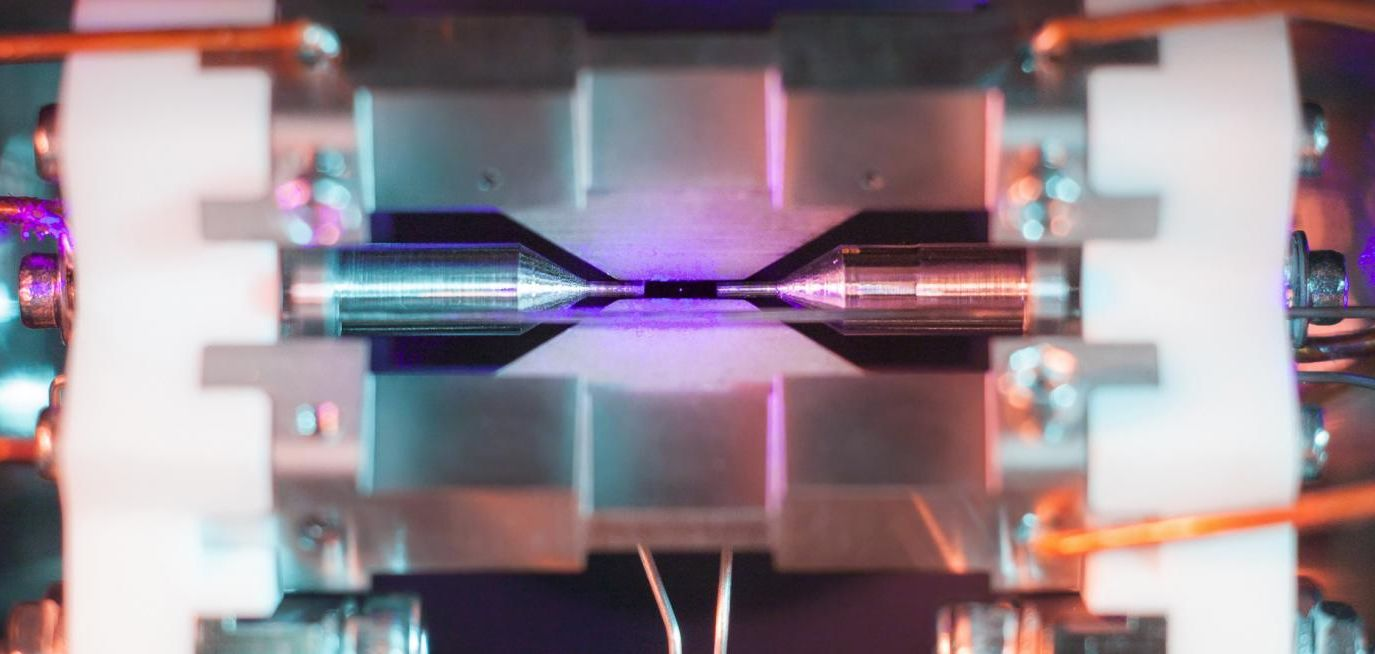
\includegraphics[width=0.95\linewidth]{TIQC.jpg}\\
			\vspace*{-.5em}\\
			\parbox{\linewidth}{\centering\footnotesize A trapped ion at the University of Oxford Ion trap quantum computing research group. Picture taken from their website\footnotemark.}
		\end{tabular}
		\vspace*{-0.75em}
	\end{wrapfigure}
	
	It is very important therefore to ensure that the qubits can be manipulated reliably. To achieve this one needs a relatively stable quantum state that can be used as the qubits and some stable way of sharing information between, manipulating and measuring these qubits to implement quantum algorithms reliably. A promising avenue toward implementation is by using trapped ions. These are charged atomic particles that are confined using magnetic and electric fields. Their internal electronic structure is ideal for use as qubits, while their back and forth motion in the trap is shared between all the ions present. As these ions are cooled to a few millionths of a Kelvin above absolute zero, this motion takes on a quantum nature, meaning that the ions' motion will only have discrete energies. This makes it a very convenient way of facilitating entanglement between them. Combination of Lasers addressing the ions can then be used to facilitate transfer between the various qubit states.
	
	In our MSci project, we simulated how different combinations of lasers, called driving schemes, can improve the reliability of a quantum computer. We did this to set expectations and give guidance to an upcoming experiment, where these schemes will be tested on a physical system. Because of this our main focus was how we can mitigate against experimental errors that inevitably arise and reduce the reliability of the qubits' state. These come from a variety of sources like the temperature and degree to which the ions can be confined. To find the best setup for the experiment we evaluated different driving schemes aimed to address the specific problems a physical system might face and have given recommendation on which ones to use. We also shown that several of these schemes could be combined giving improved performance. We hope that the increased reliability of these schemes will be demonstrated in the following years.
}
\vspace*{\fill}

\footnotetext[1]{\href{https://www.physics.ox.ac.uk/research/group/ion-trap-quantum-computing}{https://www.physics.ox.ac.uk/research/group/ion-trap-quantum-computing}}
\newpage

\fancyhead[RE,LO]{}
%%%%%%%%%%%%%%%%%%%%%%%%%%%%%%%%%%%schemes%
\newcounter{abstractpage}
\setcounter{abstractpage}{\value{page}}

\begin{abstract}
\thispagestyle{fancy}
\setcounter{page}{\value{abstractpage}}

In the present work we discuss potential entangling gate designs for a trapped ion quantum computer, utilising the $^{40}$Ca$^+$ ion's $5S_{1/2,m_j=1/2} \leftrightarrow 4D_{5/2,m_j=1/2}$ quadrupole transition as its qubit state. We give an overview and then explore effects reducing the expected fidelity in a physical implementation. The two problems we focus on are thermal effects reducing fidelity, due to high ion temperatures and unwanted off resonant transitions, which arise from strong driving, which is unavoidable in fast gates. We propose a solution to these problems by combining the strong coupling \cite{SC_Paper} and cardioid \cite{Cardioid} scheme. With this compound gate we expect an experimental infidelity of $\sim 2\cdot 10^{-5}\%$ with a gate time of $90\;\mu s$. We also show that as a first proof of concept the cardioid may be used in the compound gate's stead, as long as the system is kept reasonably cold. We further expand on a dynamical decoupling scheme presented by \cite{DD_Paper}, for use in our compound gate. We demonstrate that this can eliminate errors stemming from qubit energy shifts on the order of $1\;\mathrm{kHz}$.
	
\setcounter{abstractpage}{\value{page}}
\end{abstract}

\setcounter{page}{\value{abstractpage}}
\stepcounter{page}
\newpage
%%%%%%%%%%%%%%%%%%%%%%%%%%%%%%%%%%%%
%\section*{Acknowledgments}

\vspace*{\fill}
\begin{center}
	\textbf{Acknowledgements}\\
	I would like to acknowledge my partner, who we discussed various driving scheme combinations with. I would also like to thank my supervisor Prof Richard Thompson, as well as Simon Webster, who guided the project from the start. I would also want to extend a special thanks to Jake Lishman, who was very accommodating, when we needed to clarify a minor misunderstanding about his work.
\end{center}
\vspace*{\fill}
%Comment this out if not needed.
\newpage

\vspace*{\fill}
\begin{center}
	\textbf{Declaration of work}\\
	Since me and my partner have worked on investigating different driving schemes and sources of errors, the work presented here is predominantly my own, including any code that was used. While the theoretical work was shared, the aspects highlighted in this report and especially Section \ref{Driving_schemes:Compound}, was mostly developed by me.
\end{center}
\vspace*{\fill}
%Comment this out if not needed.
\newpage
%\clearpage{\pagestyle{empty}}

%%%%%%%%%%%%%%%%%%%%%%%%%%%%%%%%%%%%
%--- table of contents
\fancyhead[RE,LO]{\sffamily {Table of Contents}}
\tableofcontents
%\listoffigures
%\listoftables 

\clearpage{\pagestyle{empty}\cleardoublepage}
\pagenumbering{arabic}
\setcounter{page}{1}
\fancyhead[LE,RO]{\slshape \rightmark}
\fancyhead[LO,RE]{\slshape \leftmark}

%%%%%%%%%%%%%%%%%%%%%%%%%%%%%%%%%%%%
\chapter{Introduction}
\label{Intro}

Quantum computers offer interesting new avenues for many scientific disciplines. Due to their versatility many algorithms have been created for them, which vary across a variety of distinct fields. These range from computer science and cryptography with Shor's algorithm \cite{Shor}, general optimisation \cite{Quantum_optimiser} as well as variational quantum eigensolvers, which would prove useful in computational condensed matter theory \cite{VQE_CMTH}.

One promising avenue toward implementation is by utilising trapped ion systems \cite{Trapped_ion_rev,Trapped_ion_qbit_toolbox,Trapped_Quantum_Computer}. These designs benefit from relatively easy manipulation of the qubits' state, a convenient energy structure allowing the separation of readout and qubit states as well as long qubit decoherence times \cite{QIP_Trapped_ions}. This allows for theoretical quantum gates to be designed with incredible fidelity, some reporting $1-10^{-10}$ \cite{SC_Paper}.

Unfortunately these fidelities have not been demonstrated in a lab environment, due to factors the theoretical models do not account for. Despite these shortcomings hyperfine qubits have demonstrated fidelities of $99.9\%$ \cite{Hyperfine_qubit} and optical ones reaching $99.6\%$ \cite{Optical_qubit}, with superconducting qubits being the only competing quantum computer design to achieve similar performance \cite{Trapped_ion_rev}.

In this work we aim to evaluate and present recommendation for gate designs, which would be suitable to implement on a $^{40}$Ca$^+$ ion quantum computer utilising optical qubits. Our goal was to find fast and reliable gates, so we can then be give recommendation to an upcoming experiment which will attempt to implement the recommended gate designs. Our goal was to find reliable gates operating near, or under $100\;\mu s$. For this reason in the following work we mainly focus on the off resonant transitions that are inadvertently driven, by the strong fields required to operate such a fast gate. For this we used a combination of theoretical and computational work.

%%%%%%%%%%%%%%%%%%%%%%%%%%%%%%%%%%%%
\chapter{Background}
\label{Background}

\section{Radio-Frequency Trap}
\label{Background:RF_Trap}

To understand the operation of trapped ion quantum computers, we have to examine how they are implemented and what properties these systems have. The trap we are interested in is a so called radio-frequency (RF) or Paul trap \cite{RF_Traps, Charged_Particle_traps_Paul}. As pictured in \figref{fig:rftrap:schematic} this design uses several electrodes to create an oscillating potential, which induces a trapping force on charged particles, but in addition to this design many others exist \cite{Trapped_ion_rev}. The stability, design and construction of these traps is extensively documented in literature \cite{Charged_Particle_traps_Paul,RF_Traps} and because these subtleties are not important to the present work these will not be further discussed here.

To simulate the ions' dynamics we can treat the their electronic structure as a two level system with transition frequency $\omega_0$. In reality this is far from the case, and other states are expressly needed for the quantum computer's operation, such as the readout state. Thinking about our system only in terms of the qubits' however, allows us to express the Hamiltonian of many ions in a trap as \cite{RF_Traps}:

\begin{align}
	\hat{H} &= \sum_{i} \frac{\hbar \omega_0}{2}\hat{\sigma}_z^{\left(i\right)} + \hbar\nu\left(\hat{a}^\dagger\hat{a} + \frac{1}{2}\right)
	\label{eq:RF_Trap_H}\\
	\hat{H} &= \frac{\hbar \omega_0}{2}\hat{S}_z + \hbar\nu\left(\hat{a}^\dagger\hat{a} + \frac{1}{2}\right)
	\label{eq:RF_Trap_H_S}
\end{align}

The first term of course corresponds to the ions simplified energy structure. We have used $\hat{\sigma}_j^{\left(i\right)}$ to signal the $j$th Pauli matrix acting on the $i$th ion. We have also introduced $\hat{S}_j \equiv \sum_{i} \hat{\sigma}_j^{\left(i\right)}$, which is a useful shorthand. The second term then is the shared vibrational motion of the ions generated by the radio-frequency trap. Adding an array of monochromatic laser driving terms, each with frequency $\omega_j$ and wavenumber $\mathbf{k}_j$, this becomes:

\begin{equation}
	\hat{H} = \frac{\hbar \omega_0}{2}\hat{S}_z + \hbar\nu\left(\hat{a}^\dagger\hat{a} + \frac{1}{2}\right) + \sum_{j}\frac{\hbar\Omega_j}{2}\hat{\sigma}^{\left(n_j\right)}_+\left(e^{-i\left(\mathbf{k}_j\mathbf{\hat{z}} - \omega_jt\right)} + h.c.\right) + h.c.
	\label{eq:RF_Trap_H_driven}
\end{equation}

Here $\Omega_j$ is the usual definition of the Rabi frequency \cite{Foot} and the $j$th laser addresses the $n_j$th ion. We can further simplify this expression by using $\mathbf{\hat{z}} = \mathbf{z_0}\left(\hat{a} + \hat{a}^\dagger\right)$, where $\mathbf{z_0}$ is the ground state spread of the wavefunction, $\mathbf{z_0} = \langle0|\mathbf{\hat{z}}|0\rangle=\hat{e}_z\sqrt{\hbar/(4\pi m\nu)}$. Here $\hat{e}_z$ is just the unit vector pointing toward the trap's axis and $m$ is the trapped ion's mass\cite{Experiment_setup}. This can then be used to define the Lamb-dicke parameter\cite{Sideband_cooling_penning_trap} as $\eta_j\equiv\mathbf{k}_j\mathbf{z_0}$. As we will see later this is used to quantify the coupling of our laser to the trap's motional modes. Using this we can rewrite the previous Hamiltonian as:

\begin{equation}
	\hat{H} = \frac{\hbar \omega_0}{2}\hat{S}_z + \hbar\nu\left(\hat{a}^\dagger\hat{a} + \frac{1}{2}\right) + \sum_{j}\frac{\hbar\Omega_j}{2}\hat{\sigma}^{\left(n_j\right)}_+\left(e^{-i\left(\eta_j\left(\hat{a} + \hat{a}^\dagger\right) - \omega_jt\right)} + h.c.\right) + h.c.
	\label{eq:RF_Trap_H_driven_LD_param}
\end{equation}

We can then move into the interaction picture with respect to the first two terms. Defining $\hat{\tilde{a}}\equiv\hat{a}e^{i\nu t}$ and $\hat{\tilde{a}}^\dagger\equiv\hat{a}^\dagger e^{-i\nu t}$ and disregarding the fast oscillating terms we can write the new Hamiltonian as:

%\begin{wrapfigure}{r}{0.5\linewidth}
\begin{figure}[t!]
	\centering
	\begin{subfigure}[t]{0.4\textwidth}
		\centering
		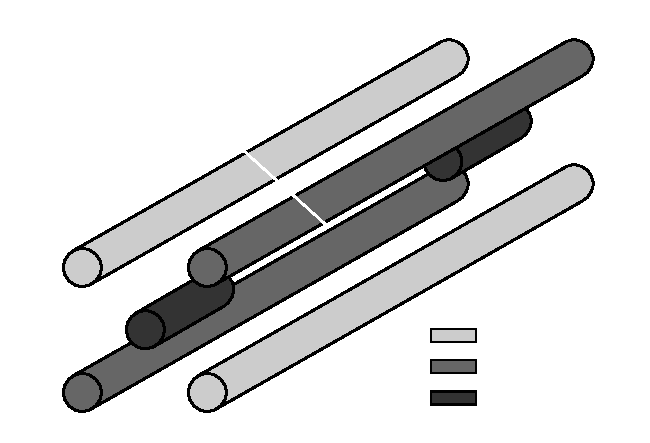
\includegraphics[width=\textwidth]{RF_Trap.pdf}
		\caption{A schematic representation of a simple RF trap. The four electrodes and two endcaps provide the trapping potential.}
		\label{fig:rftrap:schematic}
	\end{subfigure}
	\hfill
	\begin{subfigure}[t]{0.55\textwidth}
		\centering
		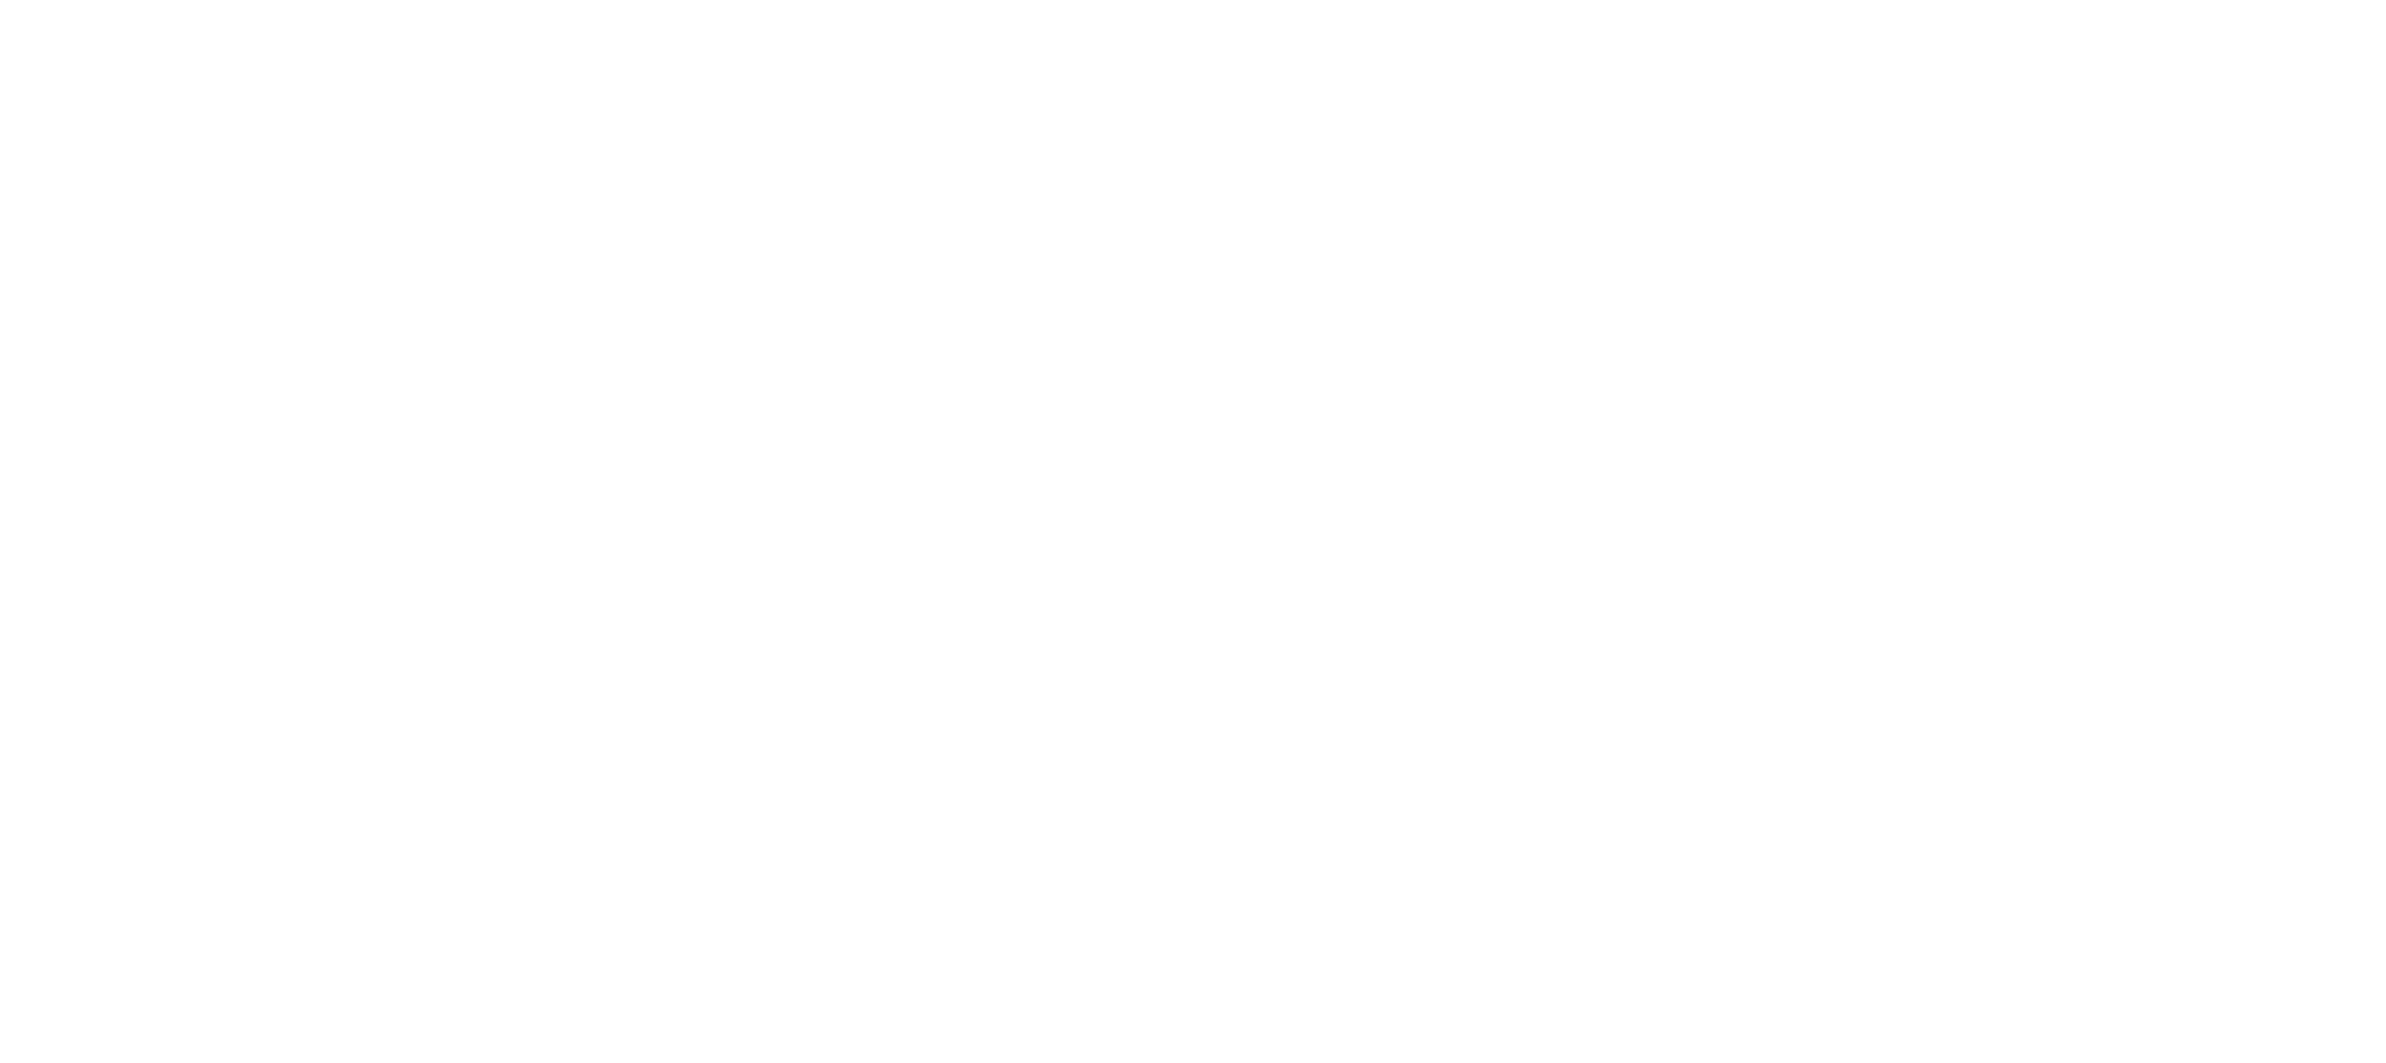
\includegraphics[width=\textwidth]{1ion_Elevels.pdf}
		\caption{Simplified energy structure of an ion in the trap. The qubit states are separated by $\omega_0$ while the motional modes' spacing is dependent on the RF trap's frequency $\nu$.}
		\label{fig:rftrap:estructure}
	\end{subfigure}
	%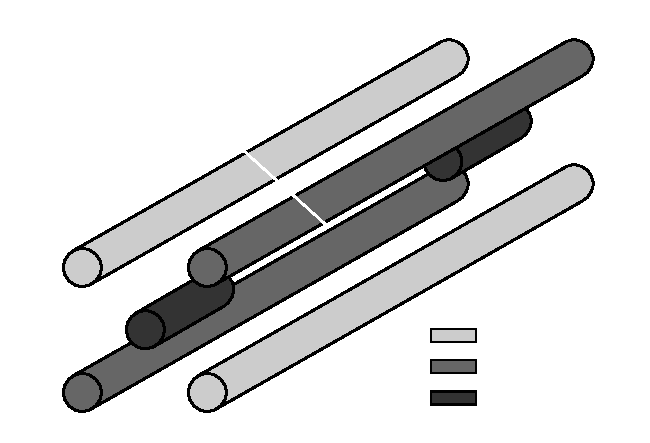
\includegraphics[width=0.7\linewidth]{RF_Trap.pdf}
	\caption[RF Trap schematic and energy]{The static field generated by the endcaps is combined with a fast oscillating field to provide confinement. This usually organises the ions on the trap's axis in a string like pattern \cite{RF_Traps,Charged_Particle_traps_Paul}. This creates an electronic structure pictured in \figref{fig:rftrap:estructure}.}
	\label{fig:rftrap}
\end{figure}
%\end{wrapfigure}

\begin{equation}
	\hat{H}_I = \sum_{j}\frac{\hbar\Omega_j}{2}\hat{\sigma}^{\left(n_j\right)}_+e^{i\eta_j\left(\hat{\tilde{a}} + \hat{\tilde{a}}^\dagger\right)} e^{-i\Delta_jt} + h.c.
	\label{eq:Interaction_H}
\end{equation}

Here we defined $\Delta_j\equiv\omega_j-\omega_0$. We can further examine this Hamiltonian by applying the Lamb-Dicke regime approximation, which is valid for $\langle\eta_j\hat{a}^\dagger\rangle \ll 1$ \cite{MS_gate}. In this limit, we can replace our exponential with the first order expansion, yielding the Hamiltonian:

\begin{equation}
	\hat{H}_I = \sum_{j}\frac{\hbar\Omega_j}{2}\hat{\sigma}^{\left(n_j\right)}_+\left(\mathds{1} + i\eta_j\left(\hat{\tilde{a}} + \hat{\tilde{a}}^\dagger\right)\right)e^{-i\Delta_jt} + h.c.
	\label{eq:Interaction_H_LD}
\end{equation}

This representation highlights two major issues about the system. The most obvious is that coupling to motional sidebands that used to share information between the ions \cite{QIP_Trapped_ions} heavily depends on the vibrational mode of the ions. This dependence will inevitably lead to decoherence of the qubit states, since the necessary timing will then differ for the various thermal occupations. This problem is further intensified by the RF trap's intrinsic property of heating \cite{QIP_Trapped_ions,RF_Traps}, which will lead to collapse of the motional mode so any entanglement of the qubits with this mode must be avoided.

The second issue is not as immediately obvious. This problem arises from the relative coupling strength of the carrier and the sideband transitions. While the central carrier transition will have coupling strength on the order of $\Omega_j$, an illuminating laser will only couple to the  $n$th sideband as an order of $\Omega_j\eta_j^n$. We will see later that this property leads to several unintended consequences, especially since $\eta_j\ll 1$ holds in most cases.

\section{M\o lmer-S\o rensen Gate}
\label{Background:MS_gate}

\begin{figure}[t!]
	\centering
	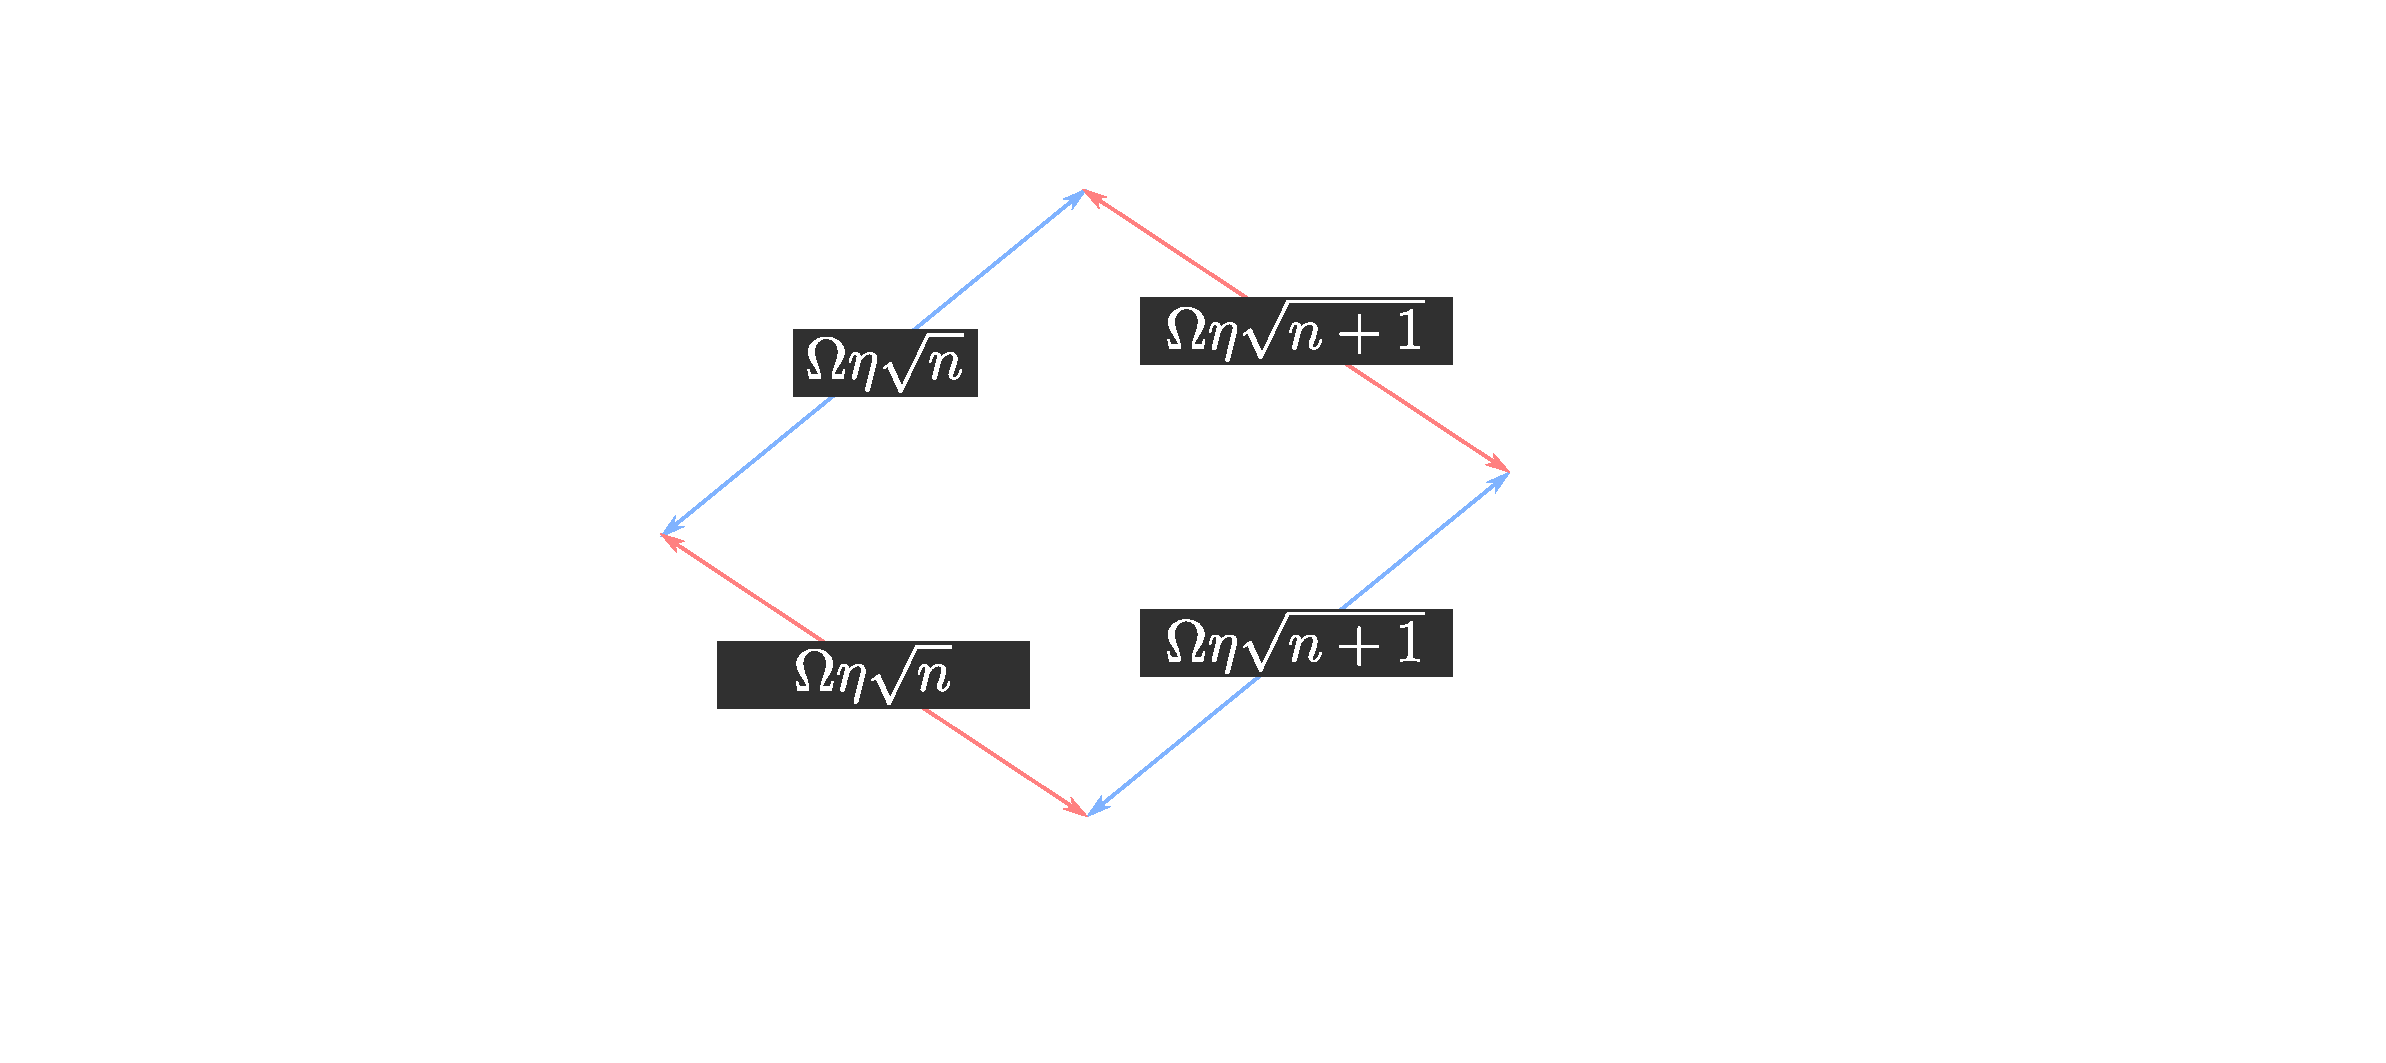
\includegraphics[width=0.9\linewidth]{MS_Gate_Schematic.pdf}
	\caption[MS-gate schematic representation]{A schematic representation of the MS-gate. The lasers drive Raman like transitions between the $|gg,n\rangle$ and $|ee,n\rangle$, through far detuned intermediate states $|eg,n\pm 1\rangle$ and $|ge,n\pm 1\rangle$. The difference in the coupling strength between the two paths available will ensure that the frequency of the transition between the ground and excited states is independent of the motional state $n$.}
	\label{fig:ms_gate_schematic}
\end{figure}

The MS gate solves the first of these problems by addressing the ions in parallel rather than in sequence, as would be standard in a Cirac-Zoller type gate \cite{Cirac_Zoller}. By driving the ions with two laser frequencies, $\Delta_1=\nu-\delta$ and $\Delta_2=-(\nu-\delta)$ simultaneously, we can drive a Raman like \cite{Foot} transition between the $|gg,n\rangle$ and $|ee,n\rangle$ levels by using $|eg,n\pm 1\rangle$ and $|ge,n\pm 1\rangle$ as intermediaries. This is pictured in \figref{fig:ms_gate_schematic}. Alternatively this can also be used to drive transitions between $|eg,n\rangle$ and $|ge,n\rangle$ as discussed within \cite{MS_gate}.

Considering the Lamb-Dicke regime and using second order perturbation theory we can then derive that the transition frequency between the two states will be $\frac{\left(\Omega\eta\right)^2}{2\left(\nu-\delta\right)}$\cite{MS_gate}. As we can see this result is independent of the occupation number $n$ therefore eliminating the gates dependence on it. Furthermore as the system is far detuned from $n\pm1$ no considerable entanglement ever occurs with the thermal state. This gate however still allows us to create an arbitrary entanglement phase between our qubits, creating a gate operation that can be characterised by $|gg\rangle\rightarrow\cos\left(\Phi\right)|gg\rangle + i\sin\left(\Phi\right)|ee\rangle$, where $\Phi$ is a phase parameter dependant on the time we allowed the system to evolve.

The condition that the lasers must be far detuned from the sideband transitions however, is a severe limiting factor in the efficiency of the gate. This requirement slows down gate operation significantly, which exposes the trapped ions to more noise than a faster gate would \cite{Trapped_ion_qbit_toolbox}. To solve these issues, the freedom in choosing $\Phi$, or the entanglement phase can be sacrificed. By allowing the system to briefly transfer population to $|n\pm 1\rangle$ we can speed up entanglement between $|gg\rangle$ and $|ee\rangle$. M\o lmer and S\o rensen have demonstrated that such a setup can be found, decreasing time taken to produce the target $\frac{1}{\sqrt{2}}\left(\left|gg\right\rangle + i\left|ee\right\rangle\right)$ significantly \cite{Fast_MS}. As this gate design is closer to what we are interested in MS gate will refer to this fast design in this thesis.

\section{Physical System}
\label{Background:PhysSys}

As mentioned this work was undertaken to set expectations for a physical implementation of the gates we will discuss in Section \ref{Driving_schemes}. The experiment we are interested in uses $^{40}$Ca$^+$ ions in a linear RF trap as described in \cite{Experiment_setup}. This paper uses the same experimental setup that will be adapted to implement quantum gates. Due to this reason, most our simulations will use the same parameters as the ones described in the paper. We are mostly interested in the trap frequency, which is set as $\frac{\nu}{2\pi} \approx 1.1\;\mathrm{MHz}$. This is so important for our gates, since it is beneficial if all driving strengths $\Omega_j$ and detunings $\Delta_j$ are expressed as a fraction of the state's separation. A slightly less, but still important parameter is the transition frequency, since it is used to calculate the Lamb-Dicke parameter.

In this project we modelled our simulations so that the $4S_{1/2,m_j=1/2} \leftrightarrow 3D_{5/2,m_j=1/2}$ transition would be our qubit state, which is a long lived qubit due to the decay being forbidden under the electric dipole selection rules \cite{Foot}, yielding a lifetime of around a second \cite{Ca_lifetime}. This transition has $\frac{\omega_0}{2\pi} \approx 411\;\mathrm{THz}$, which can then be used to calculate the Lamb-Dicke parameter for the setup, for which our figure is consistent with the one presented in \cite{Experiment_setup}. At this point for convenience a slight approximation can be made. Since all lasers would be parallel to the trap's axis, and have similar wavenumbers we have decided that to take ${\eta_j \approx \eta}$, where $\eta$ was defined as the Lamb-Dicke parameter of a laser resonant to the carrier transition. While a scheme where this assumption does not hold might be interesting to pursue, that is beyond the scope of this work. 

%%%%%%%%%%%%%%%%%%%%%%
\chapter{Simulation Framework}
\label{Sim_Framework}

To evaluate the gate designs we had to simulate realistic conditions, which we would expect to see in an experimental setting. To achieve this we decided to use Qutip \cite{QuTip1,QuTip2}, a simulational framework used to model problems relating to quantum systems. We have used their numerical solvers to integrate the von Neumann equation \cite{Shankar_QM} ${\der{\hat{\rho}}{t} = -\frac{i}{\hbar}\left[\hat{H},\hat{\rho}\right]}$, where we substituted the Hamiltonian from \eref{eq:RF_Trap_H_driven}, with of course $\rho$ marking the density matrix.

\begin{figure}[b!]
	\centering
	\begin{subfigure}[t]{0.475\textwidth}
		\centering
		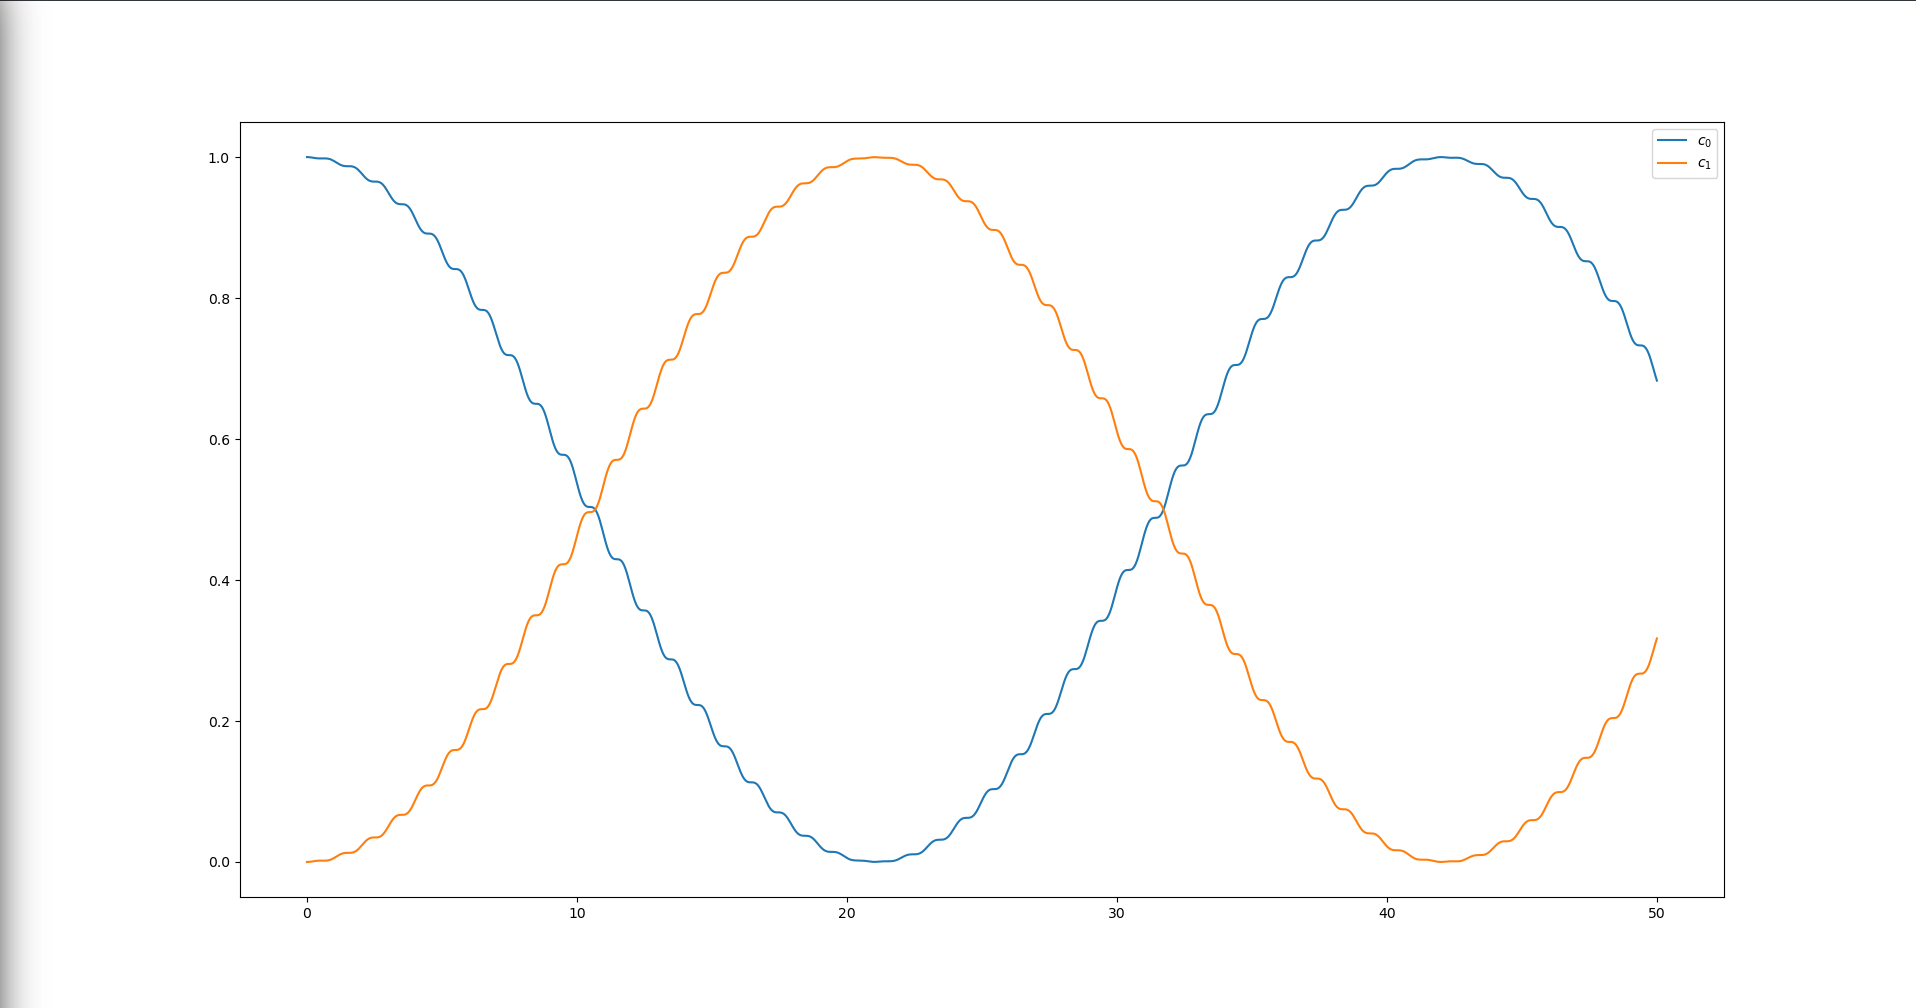
\includegraphics[width=\textwidth]{Rabi.pdf}
		\caption{Simulated two level system population in presence of a resonant driving field with Rabi frequency of $\frac{\Omega}{2\pi} = 1000\;\mathrm{Hz}$. The two levels' population is shown as the diagonal elements in the density matrix $\hat{\rho}$.}
		\label{fig:rabi:measured}
	\end{subfigure}
	\hfill
	\begin{subfigure}[t]{0.475\textwidth}
		\centering
		\includegraphics[width=\textwidth]{Rabi_residual.pdf}
		\caption{Error in the simulation as characterised by the inaccuracy of $\langle e|\hat{\rho}|g\rangle$ compared to its theoretical value. As we can see our simulation differs in a mostly negligible fashion that is expected of any numerical solution.}
		\label{fig:rabi:residual}
	\end{subfigure}
	%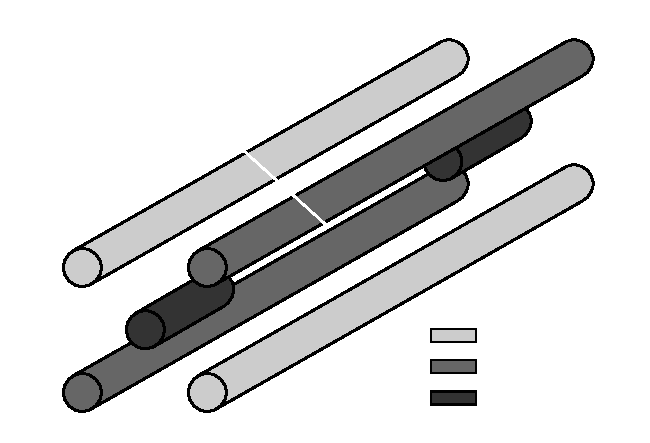
\includegraphics[width=0.7\linewidth]{RF_Trap.pdf}
	\caption[Rabi oscillation simulation]{Benchmark simulation involving Rabi oscillations. For these parameters $\langle e|\hat{\rho}|e\rangle = \sin^2\left(\frac{2\pi1000}{2}t\right)$ is expected, which is what can be observed.}
	\label{fig:rabi}
\end{figure}

To confirm that our simulation had no artefacts we decided to use two benchmarks. The first was a confirmation of the solver producing high precision data, for which a simple simulation of a Rabi oscillation was sufficient. For this result to not be tainted by motional modes we have set $\eta =0$, effectively modelling a particle without motional coupling.

The second test was designed to find bugs in the expansion of $e^{i\eta\left(\hat{\tilde{a}}+\hat{\tilde{a}}^\dagger\right)}$. Testing for the second artefact was harder since the Hamiltonian where this term is fully expanded is difficult to solve analytically. In order to circumvent this we decided to reproduce Figure 2 from \cite{MS_gate}. This allowed us to compare our simulation's performance to established work. The results of these simulations can be seen in Figures \ref{fig:rabi} and \ref{fig:msbench}.

We can see that both our simulations agree with either the theoretical prediction. In the case of the Rabi oscillation we are able to see the inaccuracies the numerical integrator introduces to our result. It is also clear that this inaccuracy is small enough not to taint our other simulations. For the MS gate's case we can not make such a precise comparison. This is due to the fact that the exact data is not available. On visual inspection however both simulations seem to match. The main features that are of interest are the slow dampening of the oscillations, the period of $T \approx 12000/\nu$ and the fast small amplitude oscillations appearing on the peak of $Re(\langle gg|\hat{\rho}|gg\rangle)$.

An other important thing to consider was the performance of our simulation. Unfortunately even though the full Hamiltonian would be preferred, sometimes simulating a system that complex would be too computationally intensive. To illustrate this we can express motional coupling of the Hamiltonian can be expanded into a form:

\begin{equation}
	e^{i\eta\left(\hat{\tilde{a}}+\hat{\tilde{a}}^\dagger\right)} = \sum_{k=-\infty}^\infty \hat{c}_k e^{-ik\nu t}
	\label{eq:Mot_exp}
\end{equation}

\begin{figure}[t!]
	\centering
	\begin{subfigure}[t]{0.475\textwidth}
		\centering
		\includegraphics[width=\textwidth]{MS_Gate_Benchmark.pdf}
		\caption{Simulation of the standard MS gate. The density matrix elements we are most interested in are plotted. The real part is displayed as a solid while the imaginary component is plotted as a dotted line.}
		\label{fig:msbench:measured}
	\end{subfigure}
	\hfill
	\begin{subfigure}[t]{0.475\textwidth}
		\centering
		\includegraphics[width=\textwidth]{MS_Gate_paper.pdf}
		\caption{The original simulation presented reproduced from \cite{MS_gate}. The solid line represents $Re\left(\langle gg|\hat{\rho}| gg\right)$, the long dashed line is $Re\left(\langle ee|\hat{\rho}|ee\rangle\right)$ and the short dashed line is $Im\left(\langle gg|\hat{\rho}|ee\rangle\right)$.}
		\label{fig:msbench:original}
	\end{subfigure}
	%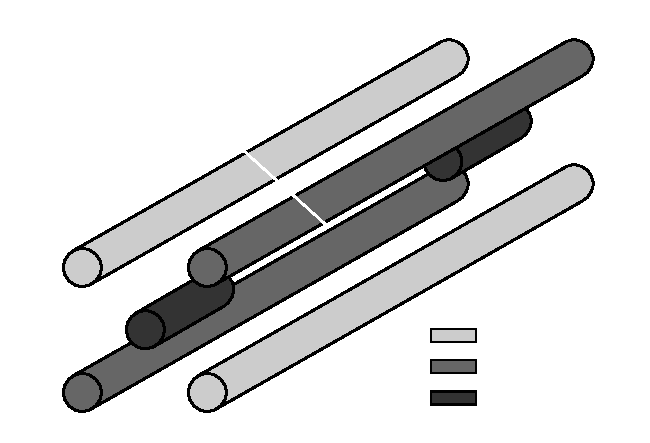
\includegraphics[width=0.7\linewidth]{RF_Trap.pdf}
	\caption[MS Gate benchmark]{Benchmark simulation reproducing Figure 2 from \cite{MS_gate}. As we can see the timing and shape of both curves are in agreement, furthermore both exhibit the same high frequency oscillations toward the peak of $\langle gg|\hat{\rho}|gg\rangle$.}
	\label{fig:msbench}
\end{figure}

Here each term represents a transition on the motional modes, with $\hat{c}_k$ facilitating a transition between $|n\rangle$ and $|n+k\rangle$. It is sometimes beneficial to consider the approximation $\langle\hat{c}_k\rangle\approx\langle\eta^k\hat{a}^{\dagger k}\rangle$. While this expression does not hold perfectly it can be a useful tool. One can arrive at this naive approximation, by expanding the exponential manually and for each diagonal only considering the first, or strongest term. While this is only a heuristic to provide us insight into computational difficulties, it is a very useful tool, when considering the relative coupling strengths, since these first terms would be dominant if $\langle\eta^k\hat{a}^{\dagger k}\rangle\ll 1$. From this it is very easy to see how small the coupling of the laser is to far off sidebands\cite{Charged_Particle_traps_Cooling}. This weak coupling issue is compounded by the fact that these far detuned transitions, will have large $|\Delta_j -k\nu|$, which will induce fast small amplitude oscillations. These only influence the end result in very minor ways, but despite this, they slow down computation significantly. One way of dealing with this is to ignore transitions, that are "off resonant", i.e. when the laser is far detuned from them, which is the tactic used by many papers on the subject\cite{Cardioid,MS_gate,Fast_MS,SC_Paper}. As we will see later this is not exactly an optimal solution since it loses valuable information about the feasibility of these gates, and is only useful when the theoretical description needs to be somewhat simplified. Instead we introduced a culling condition into our Hamiltonian:

\begin{equation}
	|k\nu-\Delta_j| > 50|\Omega_j|\cdot 2^{|k|}\eta^{|k-1|}
	\label{eq:culling}
\end{equation}

This is used so any term in \eref{eq:Mot_exp} that cannot fulfil this condition will be discarded. This expression is generous enough that for our purposes, the results are indistinguishable from a full Hamiltonian simulation. We have decided to use a cutoff of $|\Delta_j -k\nu| = 50\Omega_j$ as detuning since we observed in preliminary  tests that this produced reliable results. We also included factors of $2\eta$ to bias against far sidebands, which is a condition resulting from the naive expansion of $\hat{c}_k$ in \eref{eq:Mot_exp} for $n=4$. While we found that these parameters, and formula produced accurate results, we concede that the choice of cutoff values are somewhat arbitrary and we advise anyone to carefully evaluate this approach if used. We have monitored that no important terms were discarded. We did this, by running simulations with some parameter like $\eta$ or $\Omega$, being varied beyond the bounds of the regime we were interested in. If no sudden jumps in the fidelity graphs were observed, then we deemed the expression safe to use inside that regime.

Finally to characterise the designs we will be using the infidelity of the final state. This can be expressed as $1-\langle\Psi|\hat{\rho}|\Psi\rangle$, where $\Psi$ is the target state. This will generally be $\Psi = \frac{1}{\sqrt{2}}\left(\left|gg\right\rangle + i\left|ee\right\rangle\right)$, but as we will see later some gates allow flexibility beyond this.

The code used to run the simulations along with some of the configurations used to generate plots is made public in a repository \cite{Github} and after submission will only see minor changes like commenting and removing legacy sections. The unaltered version will be kept on the "Thesis" branch. This repository contains original code produced by the author for the purpose of simulating the fidelity of the driving schemes presented below. The simulations were produced by the three files \texttt{Seq\_core.py}, \texttt{Var\_core.py} and \texttt{Time\_core.py}. The first simulates pulse sequences and stores the evolution of the states, while the last two provide wrappers to vary some parameter about the simulation and stores only the end result.

%%%%%%%%%%%%%%%%%%%%%%%%%%%%%%%%%%%%
\chapter{Explored Driving Schemes}
\label{Driving_schemes}

\section{Strong Coupling Gate}
\label{Driving_schemes:SC}

It is clear that the motional sidebands, characterised by the exponential ${e^{i\eta\left(\hat{\tilde{a}}+\hat{\tilde{a}}^\dagger\right)}}$ play a key role in the driving scheme's fidelity. One major issue with the MS gate however is that this exponential is only very naively expanded into the Lamb-Dicke approximation\cite{Fast_MS}. While this allows for a simpler theoretical treatment of the system it fundamentally introduces errors stemming from the inaccuracies of such a treatment. An obvious solution is to include additional terms in the exponential's expansion. This is the approach taken by \cite{SC_Paper}, where an exact expansion is used in place of the simpler Lamb-Dicke approximation. Using the notation provided in \eref{eq:Mot_exp} we can represent this expansion as \cite{SC_Paper}:

\begin{equation}
	\hat{c}_k = e^{-\frac{\eta^2}{2}}\sum_{n=0}^\infty \left(i\eta\right)^{2n+k}\frac{\hat{a}^{\dagger n+k}}{\left(n+k\right)!}\frac{\hat{a}^{n}}{n!}
	\label{eq:SC_expansion}
\end{equation}

Here $k > 0$ and $\hat{c}_{-k} = \hat{c}_k^\dagger$. While this expansion is exact, there is no easy way to deal with a Hamiltonian including this. In the paper this issue is solved by iteratively computing a propagator, which is the product of several time dependent sub-propagators: $\hat{U} \approx \hat{V}_d = \prod_{n=0}^{d}\hat{U}_n$. From a propagator of this form we can generate a new Hamiltonian via the expression ${\hat{H}_{j+1} = \hat{V}_d^\dagger \hat{H}_I^{'} \hat{V}_d - i\hat{V}_d^\dagger\hat{\dot{V}}_d}$, which will only include terms until $\mathcal{O}\left(\eta^{j+1}\right)$. Here $\hat{H}_I^{'}$ is the Hamiltonian from Equation \eqref{eq:Interaction_H} without the off resonant transitions. These are ignored as including them would complicate derivation too much. This can then produce a new propagator term $\hat{U}_d = e^{-i\int_{0}^{t}\hat{H}_d\text{d}t'}$. Using the Lamb-Dicke approximation as $\hat{H}_0$ one can construct a propagator to arbitrary degrees of $\eta$\cite{SC_Paper}.

From this we can then require that, at gate time, $\hat{V}_d=e^{i\Phi\hat{S}_y^2}$, which is referred to as the entangling condition. This will ensure that our final state ${\cos\left(\Phi\right)|gg\rangle + i\sin\left(\Phi\right)|ee\rangle}$ does not have unwanted contributions from higher order terms dependant on $n$. It will also make sure that our phase will be correct when the gate operation finishes. To eliminate other terms at gate time, they utilise higher order transitions, meaning that in addition to the first sideband driving of the MS gate, they add extra terms for farther off sidebands. As an example eliminating terms with order $\eta^4$ requires driving second order, while $\eta^6$ needs third order sidebands. The expressions that need to vanish also quickly increase in both number and size as the approximation is expanded to higher order. Since these expressions are too long to be included here, we will be omitting them, but they are mentioned in \cite{SC_Paper}, with the exact conditions appearing in \cite{SC_github}. By using these higher order driving terms we can lift the Lamb-Dicke regime requirement, $\langle\eta\hat{a}^{\dagger}\rangle\ll 1$, allowing high fidelity computation with hotter states, or setups where the ions are less confined.

In the original paper discussing the design, the author provide two proof of concept driving profiles. One utilising two and an other using three sidebands. Unfortunately neither of these gates seem ideal for our purposes. This is because, when we consider terms that are off resonant their fidelity is quickly lost due to these unwanted transition. Unfortunately for fast gates on the order of $100\;\mu s$, these terms become necessary to consider. Due to this we will only be including the two sideband case, partially as a baseline for results in Section \ref{Driving_schemes:Compound}. For the or the ideal operation of these gates, as well as detailed description of the three sideband case one can refer to \cite{SC_Paper}.

\begin{figure}[t!]
	\centering
	\begin{subfigure}[t]{0.475\textwidth}
		\centering
		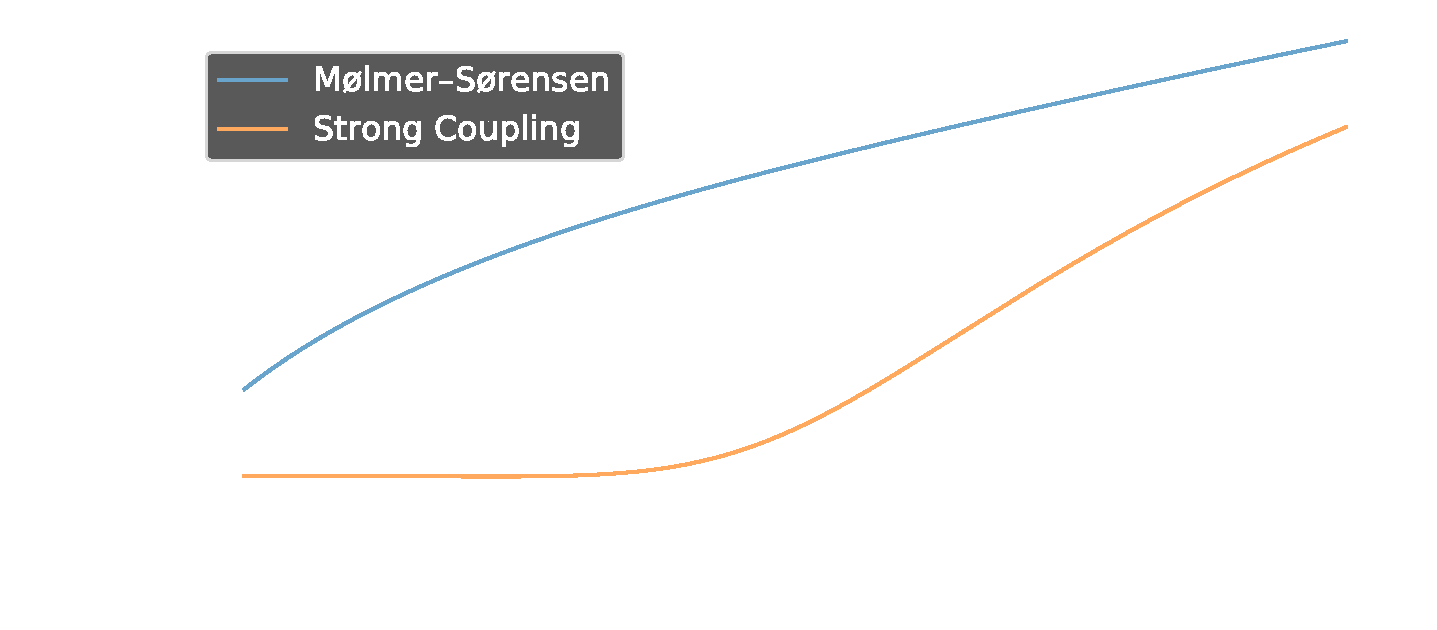
\includegraphics[width=\textwidth]{SC2_therm.pdf}
		\caption{Comparison between the MS gate and the strong coupling scheme's effectiveness against higher temperature ions, if only on resonant terms are included in the Hamiltonian. It is easily seen that the strong coupling design is more robust against these errors.}
		\label{fig:sc2:comparison}
	\end{subfigure}
	\hfill
	\begin{subfigure}[t]{0.475\textwidth}
		\centering
		\includegraphics[width=\textwidth]{SC2_off_res.pdf}
		\caption{A time scan of the strong coupling gate's operation. The initial state was set as $|gg,0\rangle$. The strong driving induces fast oscillations on the carrier, yielding fast off resonant transitions. These reduce the final fidelity to $\sim 98\%$ with the fast oscillations providing the potential to lose up to $\sim3\%$ more.}
		\label{fig:sc2:time}
	\end{subfigure}
	%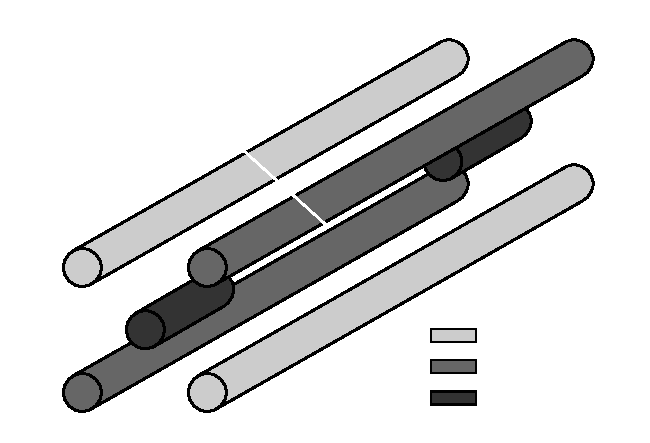
\includegraphics[width=0.7\linewidth]{RF_Trap.pdf}
	\caption[Strong coupling design]{Comparison between the effectiveness of the strong coupling gate, while only simulating on resonant (left). On the right we provide an example why this on resonant term approximation is flawed. The parameters were $\Omega_0 = 0.1\nu$ and $\Phi=0.5\pi$ for both cases, but this is more relevant to the right plot, since the left one ignores off resonant terms.}
	\label{fig:sc2}
\end{figure}

The two sideband proof of concept provided in \cite{SC_Paper} can be brought into our formulation as 4 lasers driving each of our ions. Using the definition we established in Sections \ref{Background:RF_Trap} and \ref{Sim_Framework} the parameters will be $\Delta_0 = -\Delta_1 = \nu - 2\delta$ and $\Delta_2 = \Delta_3 = 2\nu-\delta$. These lasers will have coupling strengths ${\Omega_1 = -\Omega_2 = \Omega_3 = \Omega_4 = ie^{\frac{\eta^2}{2}}\Omega}$, where $\Omega$ and $\delta$ are parameters related by the entangling condition ${3\eta^6(\frac{\Omega}{\delta})^4 - (1 + \eta^2)\eta^2(\frac{\Omega}{\delta})^2 + \frac{\Phi}{\pi} = 0}$. This will produce the expected state at gate dime defined by $t_g = \frac{2\pi}{\delta}$.

We have then compared this strong coupling gate design with the MS gate, for which the results are seen in Figure \ref{fig:sc2:comparison}. In this simulation, we highlighted the benefits of the strong coupling gate, by only considering the on resonant terms. However we can immediately see how detrimental the inclusion of these terms are, when we look at Figure \ref{fig:sc2:time}. If the gate is only weakly driven, this issue will not be present, but that comes at the cost of gate speed.

Unfortunately this design does not seem to be reasonably implementable due to these concerns about off resonant transitions. 

\section{Cardioid Gate}
\label{Driving_schemes:Cardioid}

An other design aiming to improve upon the MS gate is the cardioid family of gates. They are part of a larger ensemble of similarly designed gates, with some common properties. The idea behind their construction is that multiple tones of lasers are driven on the same sideband, which introduces further degrees of freedom that can be manipulated to produce gates that are robust against some external effects \cite{Cardioid}. In their original formulation they provide an example of resistance against timing errors.

The gates they propose have the general form $\Delta_{2i} = -\Delta_{2i + 1} = \nu - n_i\delta$, where $\delta$ is a parameter related to gate time by the familiar expression $t_g = \frac{2\pi}{\delta}$. Their relative intensities can then be expressed as $\Omega_{2i} = \Omega_{2i + 1} = r_i\Omega$, where  $\Omega = \frac{\delta}{2\eta}$ and ${\sum_{i}\frac{r_i^2}{n_i} = 1}$. They found these conditions after integrating the Lamb-Dicke regime Hamiltonian, while neglecting the off resonant carrier terms \cite{Cardioid}, similar to how \cite{SC_Paper} and \cite{Fast_MS} was designed. The proposition that off resonant terms are ignored, raises problems not unlike the ones we have seen in the strong coupling gate's case. A promising proposition is that the extra degrees of freedom we control can be used to reduce these errors.

The cardioid is a specialised version of the gate design described above. It is characterised by 2 tones on both the red and blue sidebands, with $r_0 = -r_1$ as well as a free choice of $n_0$ and $n_1$ among the integers. We can then introduce these terms into Equation \eqref{eq:Interaction_H_LD}, constructing a Hamiltonian for the treatment of off resonant transitions on the carrier:

\begin{equation}
	\hat{H}_I = \sum_j \frac{\hbar r_j\Omega}{2}(\hat{S}_x (e^{i(\nu - n_j\delta)t} + h.c.) + \eta \hat{S}_y (\hat{a}e^{in_j\delta t} + h.c))
	\label{eq:Cardioid}
\end{equation}

Where we have ignored the far resonant sideband terms, such as the red sideband detuned laser driving the blue sideband. While we could represent the propagator as $\hat{U}\approx \prod_0^t e^{-i\int_{t}^{t + \Delta t}\hat{H}_I\text{d}t'}$, the treatment and evaluation of this expression would be not only extremely laborious, but possibly fruitless as well. Due to this and the fact that this work's scope is too limited for such a discussion, we will not be pursuing this line of inquiry. 

Alternatively we can take an other, more naive approach. Instead of using the extra degrees of freedom to reduce the overall loss of fidelity that happens during gate operation, we can focus on the noise generated at gate time. This high frequency fluctuation is extremely problematic, due to it adding a randomness to the final state, with the only remedy being very precise timing. By requiring the first term to disappear at gate time, we can ensure that these unwanted transitions disappear as well. It is easy to see that for a cardioid gate, the first term can be rearranged to be proportional to $\cos(\frac{(n_0 - n_1)\delta}{2}t)$. Since $n_0, n_1 \in \mathbb{Z}$, this will ensure that at $t_g = \frac{2\pi}{\delta}$ this expression becomes zero for all cardioid type gates. These gates will also provide some resistance against timing errors as was discussed in \cite{Cardioid}.

We decided that out of the variety of cardioid gates the Cardioid($4$, $6$), would be explored, the numbers representing the values of $n_i$. As a note, since all gates in this family would be suitable for reducing off resonant carrier transitions near gate time, our choice of focusing our simulation on Cardioid($4$, $6$) was somewhat arbitrary. The reason while this specific version of the cardioid gate was included is that, this was the base that we developed into our compound gate. As all cardioid gates are similar, this is also useful to highlight the schemes beneficial properties as well as its shortcomings. Figure \ref{fig:cardioid} highlights how the cardioid scheme improves the fidelity near gate time, but does nothing to combat thermal effects. This behaviour is one that seemed to be the reverse of the strong coupling scheme.

As a final note from these measurements, it seems that, although the cardioid scheme seems to be somewhat well behaved in situations it has not been designed for. This however is probably more a property of the Lamb-Dicke regime's breakdown, than some intrinsic value of the cardioid design.

\begin{figure}[t!]
	\centering
	\begin{subfigure}[t]{0.475\textwidth}
		\centering
		\includegraphics[width=\textwidth]{Card_time.pdf}
		\caption{Simulation the full expansion of the Hamiltonian. As we can see both gates present with oscillations far from gate time, but in the case of the cardioid, this oscillation disappears stabilising the curve around $0.1\%$ infidelity. The MS gate however remains oscillating introducing a possible loss in fidelity of $\sim 2\%$ if the gate time is implemented slightly incorrectly. Both systems started in $|gg,0\rangle$.}
		\label{fig:cardioid:full}
	\end{subfigure}
	\hfill
	\begin{subfigure}[t]{0.475\textwidth}
		\centering
		\includegraphics[width=\textwidth]{Card_therm.pdf}
		\caption{Fidelity comparison between the \mbox{Cardioid($4$, $6$)} and MS gates under different ion temperatures. For the results to be without noise, we have ignored off resonant terms. As we can see the cardioid still suffers from the same loss of fidelity that is prevalent in the MS gate's case.}
		\label{fig:cardioid:therm}
	\end{subfigure}
	%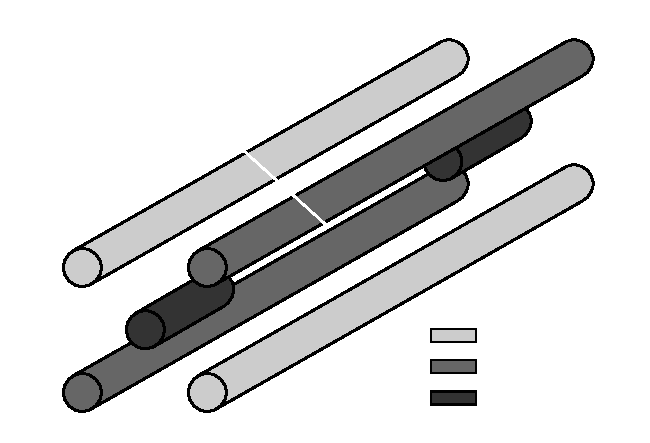
\includegraphics[width=0.7\linewidth]{RF_Trap.pdf}
	\caption[Cardioid gate comparison]{Comparison between the fidelity the MS gate and the Cardioid($4$, $6$). The left plot highlights the improvement the cardioid scheme has in a strongly driven ($\Omega = 0.1\nu$) case. The right plot however shows that since it does not expand the Hamiltonian to high orders, it is not resistant against thermal effects.}
	\label{fig:cardioid}
\end{figure}

\section{Compound Gate}
\label{Driving_schemes:Compound}

Finally we have aimed to create a gate design that has the benefits of both the strong coupling and the cardioid scheme. For this end we have used the expansion detailed in Section \ref{Driving_schemes:SC}. To efficiently utilise it, we have created a wrapper around the conditions provided in \cite{SC_github}. This allowed us to feed it parametrised versions of driving terms using Mathematica, for which the code is included in \texttt{SC2.nb}\footnote{Note that while the present work uses the same notation throughout for consistency, this file uses the framework used by \cite{SC_Paper}, since the constraints were provided in the same framework.}. To create our desired gate design the first sideband was set to mimic the target driving scheme, while the second sideband was used to reduce the necessary terms in our equation to zero. While an automatic solver for this would be preferred our solution was semi-manually. There also does not seem to be a simple way of automating the parts, which had to be done by hand, which were mostly inputting the initial ansatz to the second order sideband driving terms. This also did not produce compound schemes for all gates we tried. As an example, we have originally experimented with a Cardioid($2$, $3$) gate, however we could not find a second sideband driving, which would reduce the unwanted propagator terms to zero. We theorised that one might exist, but it seemed that for that particular driving, a lot of tones would be needed on the second sideband. Calculation of a many terms however, slowed down the process too much, prompting us to abandon the Cardioid($2$, $3$) design.

\begin{table}[t!]
	\centering
	\begin{tabular}{c||cccc|cc}
		\hline
		$\Delta_i$ & $\nu - 4\delta$ & $-(\nu - 4\delta)$ & $\nu - 6\delta$ & $-(\nu - 6\delta)$ & $\pm(2\nu - \delta)$ & $\pm(2\nu - 3\delta)$ \\
		\hline
		$\Omega_i$ & $\Omega'$ & $-\Omega'$ & $\Omega'$ & $-\Omega'$ & $\sqrt{\frac{5}{8}}\Omega'$ & $-\sqrt{\frac{5}{8}}\Omega'$\\
		\hline
	\end{tabular}
	\caption{The relative driving strengths and detunings required for the compound gate's operation. We have defined $\Omega' = ie^{\frac{\eta^2}{2}}\Omega$ for a more compact description. This design eliminates the off resonant carrier transitions from both the first and second sideband terms.}
	\label{tab:Compound}
\end{table}

\begin{figure}[b!]
	\centering
	\begin{subfigure}[t]{0.475\textwidth}
		\centering
		\includegraphics[width=\textwidth]{Compound_time.pdf}
		\caption{A comparison between the fidelities of the Cardioid($4$, $6$) and our compound gate. As we can see both fulfil their roles in reducing the gate time off resonant transitions. The compound gate is quite a bit more noisy, which is most definitely due to the extra lasers driving the transition.}
		\label{fig:compound:time}
	\end{subfigure}
	\hfill
	\begin{subfigure}[t]{0.475\textwidth}
		\centering
		\includegraphics[width=\textwidth]{Compound_therm.pdf}
		\caption{Fidelity plot showing that our compound gate retains the strong coupling gate's resistance against thermal effects. As with the other plots showing dependence on the thermal occupation $\overline{n}$ only on resonant terms were considered.}
		\label{fig:compound:therm}
	\end{subfigure}
	%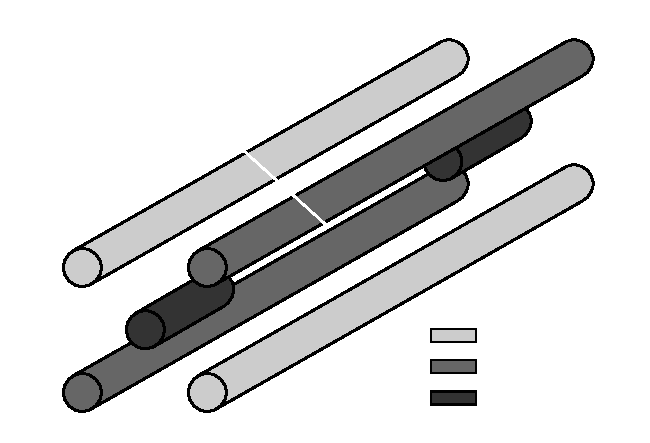
\includegraphics[width=0.7\linewidth]{RF_Trap.pdf}
	\caption[Cardioid gate comparison]{Evaluation of the compound gate. On the left we highlight its ability to reduce off resonant transitions near gate time, while on the right we show its robustness against thermal effects. As with other simulations $\Omega_0=0.1\nu$}
	\label{fig:compound}
\end{figure}

Due to the manual nature of this parameter variation, we also decided that three sideband driving cases would not be attempted. This decision was also made mainly due to computational limitations. This is because three sideband driving would require a staggering number of terms to become zero, compared to the $12$, which is needed for a two sideband design. We also believed that a three sideband gate would not improve the final gate's fidelity drastically as the extra driving terms would possibly create more noise from off resonant transitions. This however is only speculation on trends noticeable in Figure \ref{fig:comparison}. In it we can see that even though the strong coupling should outperform the MS gate, it only starts approaching a similar level of fidelity as the driving term becomes weaker, which reduces the prevalence of off resonant transitions these designs do not mitigate against. An example of this would be a second sideband laser driving a first sideband transition off resonantly.

The gate we have found a working extension for using the strong coupling constraints was the Cardioid($4$, $6$). Using $4$ lasers that were adapted in minor ways from their description in Section \ref{Driving_schemes:Cardioid} and adding a $4$ extra driving terms on the second sideband would reduce the unwanted terms in the propagator to zero. The driving scheme's breakdown can be found in Table \ref{tab:Compound}. The two tones on the second sideband was not actually needed to fulfil the strong coupling conditions and as it turns out one tone on the second sideband would have been enough. Including this extra tone however allowed us to treat the second sideband tones similar to the first, yielding a degree of freedom. By requiring that the two tones must have the same driving strength, but opposite values allowed us to eliminate off resonant carrier transitions stemming from the second sideband driving as well. For this design the entangling condition relating $\delta$ and $\Omega$ will be:

\begin{equation}
	\frac{5}{72}\left(7\eta^6\left(\frac{\Omega}{\delta}\right)^4-12\eta^2\left(1+\eta^2\right)\left(\frac{\Omega}{\delta}\right)^2\right) + \frac{\Phi}{\pi} = 0
	\label{eq:compound_entangling}
\end{equation}

With the gate time remaining at its original definition $t_g = \frac{2\pi}{\delta}$. As we can see in Figure \ref{fig:compound}, this gate combines the desired qualities of the cardioid and strong coupling schemes. It is important to note however that the off resonant transitions seem to be more intensive in the compound gate's case compared to the pure cardioid. We believe this is a combination of two properties of the system. Since the cardioid cannot achieve the same low infidelities, the logarithmic plot possibly skews the perception of the results. However the extra lasers addressing farther off sidebands, may also contribute to this noise, due to the fact that we only made carrier transitions interfere destructively at gate time, not off resonant sideband transitions.

\section{Comparison}
\label{Driving_schemes:Comparison}

To evaluate which driving scheme is the most promising candidate for implementation, we have decided to set up an array of simulations. We would then vary two parameters in these, $t_g$ and $\overline{n}$. Reducing gate time would require stronger driving yielding unwanted off resonant transitions, while increasing the thermal state would start to break down the Lamb-Dicke approximation, but would allow to simulate non-ideal conditions.

The results pictured in Figure \ref{fig:comparison} are somewhat expected. The MS and strong coupling gates are not designed for such intensive driving and therefore at these driving strengths they become unsuitable candidates. This issue is more prevalent in the strong coupling case due to the additional lasers included to reduce errors arising from thermal noise.

\begin{figure}[t!]
	\centering
	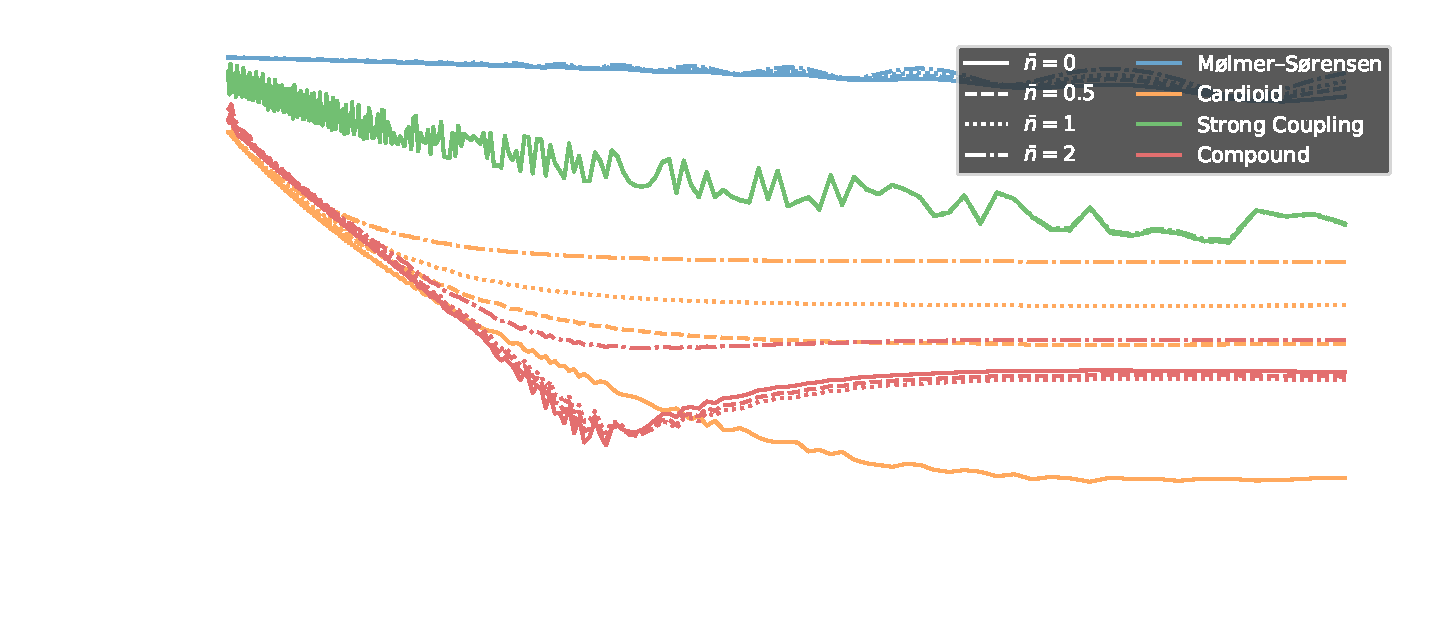
\includegraphics[width=0.9\linewidth]{Comparison.pdf}
	\caption[Gate comparison]{Comparison between the various driving schemes. The colour indicates the type of gate, while its drawing style shows the initial thermal occupation simulated. As we can see both the MS and the strong coupling gates suffer from large fluctuations in fidelity, most likely due to off resonant carrier transitions. The compound and cardioid schemes have minor noise visible as well, and these are most likely due to off resonant transitions on some sideband. Since the driving terms couple to the sidebands less strongly, their perturbation is much weaker.}
	\label{fig:comparison}
\end{figure}

The two best functioning ones are the cardioid and the compound design. It is quite interesting that the cardioid seems to outperform the compound gate above $110\;\mu s$. This peculiarity is further compounded by the minimum the compound gate's fidelity curve produces. As of yet we have not found a satisfactory explanation to the shape of this curve. An obvious cause would be the culling condition \eqref{eq:culling}, however a breakdown in that would show as a violent discontinuity in rather than a slowly stabilising fidelity curve. It is however possibly the second sideband's driving becoming less prevalent, and therefore it's negative effects would start to become less pronounced.

The cardioid gate however also has its own flaws, as evident from the quick loss of fidelity when the thermal state $\overline{n}$ is increased. This is not noticeable as strongly on the other designs, but this is mostly due to either the design mitigating against this problem like the compound gate, having an error source, which produces larger infidelities like in the case of the MS gate or possessing both these qualities like the strong coupling gate.

\section{Dynamical Decoupling}
\label{Driving_schemes:DD}

Finally I would like to talk about an addition to the previous schemes. Dynamical decoupling can be used to eliminate infidelity from errors in the qubits' transition frequencies. These drifts in qubit energy arise naturally from electric and magnetic interferences inducing Zeeman and Stark shifts \cite{Foot}. One can include any error that would shift the energy level of the qubit as an extra term in the Hamiltonian as:

\begin{equation}
	\hat{H}_I' = \hat{H}_I + \sum_i \frac{\hbar \xi_i}{2} \hat{\sigma}_z^{\left(i\right)}
	\label{eq:qubit_err}
\end{equation}

Where $\xi_i$ is the error in the $i$th qubit's frequency. As expected these errors are capable of disrupting our gate operation even with a small $\xi_i$. However by including a strong carrier driving term in the form $\frac{\hbar \Omega_c}{2}\hat{S}_y$, which was modelled after the one used in \cite{DD_Paper}, we can mitigate these problems. We can then move into the interaction picture with respect to this new term, to find that:

\begin{equation}
	\hat{H}_I'' = \hat{H}_I + \sum_i \frac{\hbar \xi_i}{2}\left(\hat{\sigma}_z^{\left(i\right)}\cos\left(\Omega_c t\right) + \hat{\sigma}_x^{\left(i\right)}\sin\left(\Omega_c t\right)\right)
	\label{eq:qubit_err_I}
\end{equation}

\begin{figure}[b!]
	\centering
	\includegraphics[width=0.9\linewidth]{DD.pdf}
	\caption[Dynamical Decoupling]{Difference between gate fidelity if the dynamical decoupling correction term is not used compared to when $\Omega_c=\nu$. Here we set $\xi_1 = \xi_2 = \xi$. We can clearly see that while the original gate quickly loses fidelity, the dynamically decoupled gate maintains it throughout, above the desired $6300\;s^{-1}$. Due to performance bottlenecks, we had to limit ourselves to simulating the on resonant terms only. The gate we used to simulate this with is the compound gate discussed in Section \ref{Driving_schemes:Compound}.}
	\label{fig:DD}
\end{figure}

This will however only be the case if $[\hat{H}_I,\hat{S}_y]=0$, otherwise our gate operation will not be unaffected by the addition of this new term. This adaptation of the driving term provided in \cite{DD_Paper} commutes with both our compound and the strong coupling gates. For the M\o lmer-S\o rensen and cardioid gates the original driving term can be used to produce equivalent results, detailed in the original paper \cite{DD_Paper}. We can also see that for $t_g, \xi_i \ll \Omega_c$ the error term reduces to fast oscillations. This will allow us to ignore it when dealing with the Hamiltonian.

One issue to be aware of however is that this Hamiltoinan will only coincide with the lab frame Hamiltonian, if $\Omega_c t_g = 2\pi n$ for $n \in \mathbb{Z}$. While it might cause a problem if this condition was not perfectly implemented, there is an other way of ensuring that the theoretical and Lab frames will match.  As discussed in \cite{DD_Paper}, if the gate is implemented as two equivalent gate operations and applying a $\pi$ pulse between them, then any partial oscillations will be refocused. This condition can be implemented easily on the compound and strong coupling gates, but some cardioid gates, might also be capable of this.

In the case of the strong coupling and compound gate designs this "split" gate can be implemented by performing two gates, each of which having a target phase $\Phi$, one which is half the original goal. This unfortunately will have the side effect of halving the gate's speed. On a larger system, this may be solved, if the two gates were actually disjunct operations that always meant to run in sequence. If both are designed to have the same gate time, then the same $\pi$ pulse may be applied between them. One interesting proposition would be to study whether, and under what circumstances can the strong coupling, compound and cardioid gates be split into two parts.

Our aim was to demonstrate that noise on the order of $1000\;\mathrm{Hz}$ or $\sim 6300\;s^{-1}$, can be eliminated using this method. By implementing the Hamiltonian in Equation \eqref{eq:qubit_err_I}, we could accurately simulate how the dynamical decoupling scheme maintains the high fidelity required, compared to the standard compound gate as can be seen in Figure \ref{fig:DD}.

%%%%%%%%%%%%%%%%%%%%%%%%%%%%%%%%%%%%
\chapter{Conclusion}
\label{Conclusion}

Out of the driving schemes we considered here, we believe that the compound design, combining the cardioid and the strong coupling gates would be the most worthwhile to explore. This design allows for resistance against both thermal effects and reduces the impact of off resonant transitions, which would hinder the performance of fast gates. This proposed gate design would also allow infidelities as low as $\sim 2\cdot10^{-5}\%$ with speeds as fast as $90\;\mu s$ according to our simulations. This high fidelity however may not be reachable by the experiment following this work, due to some unforeseen source of infidelity we did not include. Even if that were to become the case the work done here could still be used as an examination of mostly errors arising from off resonant driving terms.

The second gate to which attention should be paid is the cardioid gate. Our evaluation of the Cardioid($4$, $6$) suggest that under the right conditions it can create a state with similar fidelity to the compound case. The benefit of this design is that it only uses $4$ lasers instead of the $8$ required for our compound gate. It was also the only design, which showed that as long as the temperature was kept low it could reliably perform below infidelities of $10^{-4}$, on a $100\;\mu s$ timescale, matching our compound gate. This design however strongly suffers from issues pertaining to temperature and as such care must be taken to operate it as close to the ground state motional mode as possible, since even small increases in temperature will affect the fidelity of the final state greatly.

The strong coupling gate and the MS gate unfortunately does not perform well under the extremely strong driving that would be required to reduce the gate time to the $100\;\mu s$ range and as such they would be best explored in a slower regime, where off resonant transitions are weak. We therefore recommend that if these were to be tested, it should be done as a slower gate.

We have also explored the a dynamical decoupling scheme, which is an addition to several other gates. We demonstrated that a modified version of the original idea from \cite{DD_Paper} can be used to reduce qubit errors in the strong coupling as well as compound gates. We have demonstrated theoretically that this modification does not interfere with the compound and strong coupling designs.

Finally we have identified several key points that can be expanded upon. While our formulation to the problem of off resonant transitions solves some of the major problems associated with them, it does not address the key question of whether a gate where the off resonant transitions are suppressed could be formulated. An other possible continuation of the work is to extend the compound gate to include further terms for greater flexibility in optimising the gate. This can be both additional tones, or additional sidebands. This however would probably require a more robust computational system that would be able to find second, or even third order sideband terms given any first order driving pattern. This would greatly increase the flexibility of the produced gates and allow for more customisation. A more in-depth analysis of the interplay between the gates mentioned and the dynamical decoupling scheme might also be fruitful.



%% bibliography
\bibliographystyle{ieeetran}
\bibliography{sources}

\end{document}